%%%%%%%%%%%%%%%%%%%%%%%%%%%%%%%
%% Folie: DataGen            %%
%%%%%%%%%%%%%%%%%%%%%%%%%%%%%%%

\begin{frame}
    \frametitle{Data Generation}

\vspace*{1cm}
\begin{multicols}{2}
    Airfoil shapes are provided by the UIUC database

    Reynolds number: $[0.5, 5] \cdot 10^6$ (highly turbulent)

    Angle of attack: $[-22.5, 22.5]$

    Ground truth generated with OpenFOAM \newline (pressure, x velocity, y velocity)
    
    Training data resolution: $3\times 128 \times 128$ \newline
    (Inference region $128 \times 128 <$ full simulation domain)
    \vfill\columnbreak
    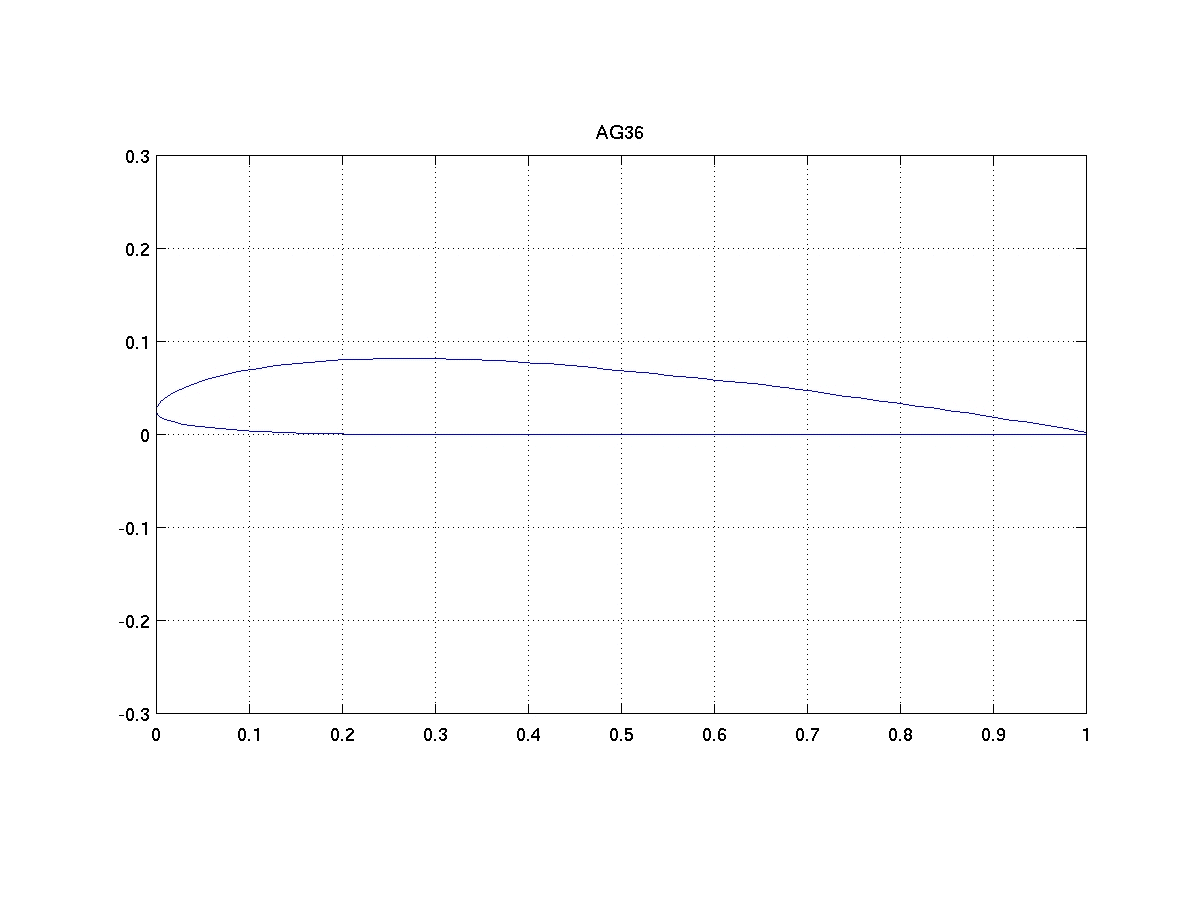
\includegraphics[width=\columnwidth, height=.6\textheight]{./Ressourcen/Praesentation/Bilder/uiuc_sample.png}
    
\end{multicols}
	\vspace*{-1.4cm}
    Taken from \url{https://m-selig.ae.illinois.edu/ads/afplots/ag35.gif}
\end{frame}
\clearpage